\rchapter{Simulation}

\section{Method Summary}

Once all the steps have been written the complete algorithm can be assembled. Memory is allocated for the distribution function $f$, the electric potential $phi$ and the perturbed charge density $rho$. Each of these objects has associated layouts. The layouts used for the distribution function can be seen in table \ref{tab::Ordering f}. The layouts used for $phi$ and $rho$ can be seen in table \ref{tab::Ordering phi}.

\begin{table}[ht]
\centering
 \begin{tabular}{|c|c|}
  \hline
  Accessing scheme & Ordering\\
  \hline
  flux\_surface & $(r,v_\parallel,\theta,z)$\\
  \hline
  v\_parallel & $(r,z,\theta,v_\parallel)$\\
  \hline
  poloidal & $(v_\parallel,z,\theta,r)$\\
  \hline
 \end{tabular}
 \caption{\label{tab::Ordering f} The chosen ordering for $f$ (the distribution function) with ($n_1$,$n_2$,1,1) processes used for the respective dimension}
\end{table}

The 3D grids have layouts that are distributed in both one and two dimensions. When the data is distributed in one dimension the data is copied across the processes. It is therefore simple to change from a layout distributed in one dimension to a similar layout distributed in two dimensions as it is simply a matter of restricting the data to the area of interest. In the opposite direction a MPI allgather command is required.

\begin{table}[ht]
\centering
 \begin{tabular}{|c|c|c|}
  \hline
  Accessing scheme & Ordering & Number of processes per dimension\\
  \hline
  v\_parallel\_2d & $(r,z,\theta)$ & ($n_1$,$n_2$,1)\\
  \hline
  mode\_solve & $(\theta,z,r)$ & ($n_1$,$n_2$,1)\\
  \hline
  poloidal & $(z,\theta,r)$ & ($n_2$,1,1)\\
  \hline
  v\_parallel\_1d & $(r,z,\theta)$ & ($n_1$,1,1)\\
  \hline
 \end{tabular}
 \caption{\label{tab::Ordering phi} The ordering for $phi$ (the electric displacement) and $rho$ (the perturbed charge density). $n_1$ and $n_2$ are the number of processes along which the first and second dimension of the distribution function are distributed}
\end{table}

The resulting algorithm is as follows:

\begin{enumerate}
 \item Compute $\tilde{\phi}$ from $f^n$ by solving the quasi-neutrality equation \ref{eq::quasi neutrality} \label{get phi}
 \begin{enumerate}
  \item Find the charge perturbation density $\rho_1$ by integrating the perturbed density function with respect to $v_\parallel$ : $\int (f-f_{eq}) dv_\parallel$
  \item Get the Fourier transform of the charge perturbation density $\rho_1$ : $\hat{\rho}_1$
  \item Set the layout of $rho$ and $phi$ to `mode\_solve'
  \item Solve the quasi-neutrality equation using the finite elements method in Fourier space to obtain the Fourier transform of the electric potential : $\mathcal{F}\left[\tilde{\phi}\right]$
  \item Set the layout of $rho$ and $phi$ to `v\_parallel\_2d'
  \item Get the inverse Fourier transform of the electric potential $\mathcal{F}\left[\tilde{\phi}\right]$ : $\tilde{\phi}$
 \end{enumerate}
 \item Set the layout of $f^n$ to `flux\_surface'
 \item Save the values in $f^n$ to a buffer
 \item Compute $f^{n+\frac{1}{2}}$ using Lie splitting
 \begin{enumerate}
  \item Carry out a flux surface advection half step
  \item Set the layout of $f^n$ to `v\_parallel' and the layout of $phi$ to `v\_parallel\_1d'
  \item Carry out a v parallel advection half step \label{v parallel step}
   \begin{enumerate}
    \item For each point along r:
    \begin{enumerate}
    \item Calculate the parallel gradient of $\tilde{\phi}$ : $\grad_\parallel \tilde{\phi}$ and save the spline representation of the result
    \item Carry out a v parallel advection half step at each point with the given value of r
   \end{enumerate}
   \end{enumerate}
  \item Set the layout of $f^n$ and $phi$ to `poloidal'
  \item Carry out a poloidal advection half step \label{poloidal step}
  \begin{enumerate}
   \item For the first value in the $v_\parallel$ direction:
   \begin{enumerate}
    \item Calculate and store the spline representation of $\tilde{\phi}$ for each point along the $z$ direction
    \item Carry out a poloidal advection half step for each point with the given value of $v_\parallel$
   \end{enumerate}
   \item For the remaining values in the $v_\parallel$ direction : Use the stored spline representations to carry out a poloidal advection half step for each point with the given value of $v_\parallel$
  \end{enumerate}
 \end{enumerate}
 \item Set the layout of $f^{n+\frac{1}{2}}$ to `v\_parallel'
 \item Compute $\tilde{\phi}$ from $f^{n+\frac{1}{2}}$ by solving the quasi-neutrality equation again using the method in point \ref{get phi}
 \item Restore the values of $f^{n}$ from the buffer thus reverting to layout `flux\_surface'
 \item Compute $f^{n+1}$ using Strang splitting
 \begin{enumerate}
  \item Carry out a flux surface advection half step
  \item Set the layout of $f^n$ to `v\_parallel' and the layout of $phi$ to `v\_parallel\_1d'
  \item Carry out a v parallel advection half step as described in point \ref{v parallel step}
  \item Set the layout of $f^n$ and $phi$ to `poloidal'
  \item Carry out a {\bf full} poloidal advection step as described in point \ref{poloidal step}
  \item Set the layout of $f^n$ to `v\_parallel'
  \item Carry out a v parallel advection half step
  \begin{enumerate}
    \item For each point along r:  Carry out a v parallel advection half step at each point with the given value of r using the saved value of $\grad_\parallel \tilde{\phi}$
  \end{enumerate}
  \item Set the layout of $f^n$ to `flux\_surface'
  \item Carry out a flux surface advection half step
 \end{enumerate}
\end{enumerate}

\section{Numerical Results}

The parameters used are the same as those in the paper by Latu et al. \cite{YamanPaper}, namely:
\begin{align*}
 & B_0=1, && R_0 = 239.8081535, &&& r_{\min}=0.1, &&&& r_{\max}=14.5,\\
 & r_p = \frac{r_{\min}+r_{\max}}{2}, && \epsilon = 10^{-6}, &&& \kappa_{n_0}=0.055, &&&& \kappa_{T_i}=\kappa_{T_e}=0.27586,\\
 & \delta_{r_{T_i}}=\delta_{r_{T_e}}=\frac{\delta_{r_{n_0}}}{2} = 1.45, && \delta_r = \frac{4\delta_{r_{n_0}}}{\delta_{r_{T_i}}}, &&& v_{\max}=7.32 
\end{align*}

The grid size is as follows:
\begin{align*}
 & N_r = 256 && N_\theta = 512 &&& N_z = 32 &&&& N_{v_\parallel} = 128
\end{align*}

The simulation also uses the following parameters:
\begin{align*}
 &\iota=0 && m=15 &&& n=1
%  &\iota=0.8 && m=15 &&& n=-11
\end{align*}

\begin{figure}[ht]
 \begin{subfigure}[t]{.5\textwidth}
  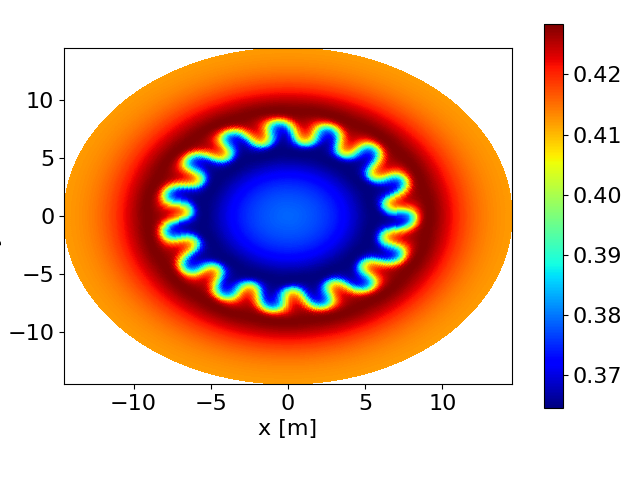
\includegraphics[width=\textwidth]{Figs/SimResults/t4000}
  \caption{T=4000}
 \end{subfigure}
 \begin{subfigure}[t]{.5\textwidth}
  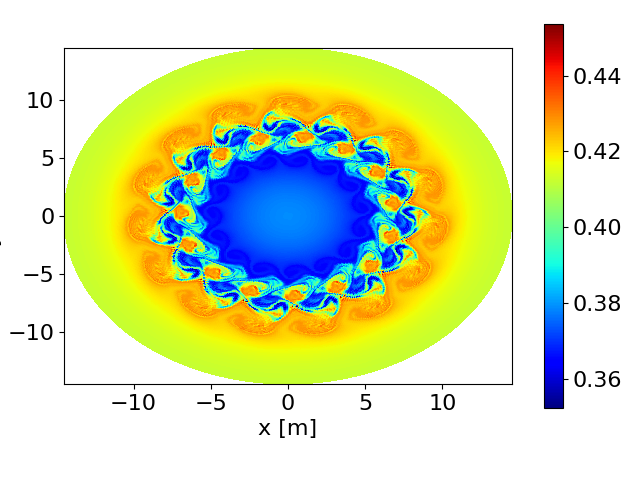
\includegraphics[width=\textwidth]{Figs/SimResults/t6000}
  \caption{T=6000}
 \end{subfigure}
 \caption{\label{fig::poloidal slice} Poloidal cut of the distribution function at different times at z=0 and $v_\parallel\approx0$}
\end{figure}

The equilibrium function as well as the radial profiles \{$T_i$ , $T_e$ , $n_0$ \} are defined in the paper by Latu et al. \cite{YamanPaper}.

The simulation results can be seen in figure \ref{fig::poloidal slice}. 


In addition to the poloidal slice the time evolution of the discrete L$^2$-norm of the electric potential is used as a diagnostic quantity. This norm is defined as follows:
\begin{equation}
 \left|\phi\right|_2(t):=\sqrt{\int_{r=r_{\min}}^{r=r_{\max}}\int_{\theta=0}^{\theta=2\pi}\int_{z=0}^{z=2\pi R_0}\phi(t,r,\theta,z)^2r\, dr\, d\theta\, dz}
\end{equation}

A trapezoidal rule is used to approximate the value. The results can be seen in figure \ref{fig::l2 phi}.

\begin{figure}
 \centering
 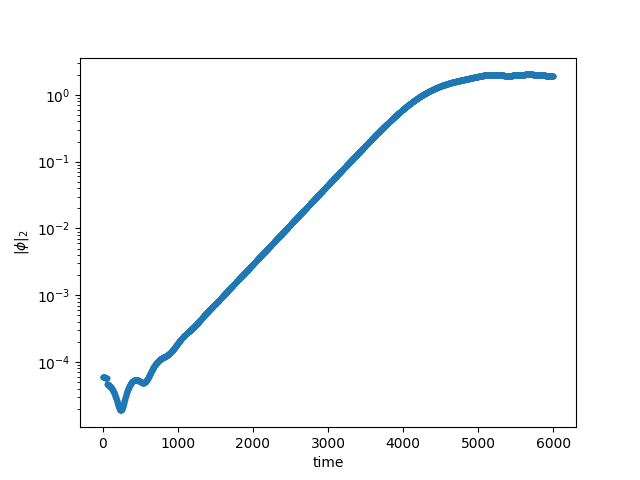
\includegraphics[width=.7\textwidth]{Figs/SimResults/l2}
 \caption{\label{fig::l2 phi}The time evolution of the discrete L$^2$-norm of the electric potential}
\end{figure}

We see that the L$^2$ norm demonstrates a linear phase as expected.
Unfortunately the gradient seen in this region is not what is expected. In addition while the poloidal planes demonstrate a similar shape to those seen by Latu et al. there appears to be some missing turbulence. We therefore conclude that the code still requires some debugging. Unfortunately time restrictions did not allow this step to be completed in time. The results so far are however close enough to the expected result to imply that it is possible to generate an accurate scientific code using this method.
% The gradient observed is in accordance with the dispersion relation as was the case for Latu et al. \cite{YamanPaper}. In addition the poloidal planes closely resemble those presented in their results. We therefore conclude that this code functions as expected and generates valid scientific results.


